%%
%% This is file `main.tex' based on `sample-sigconf.tex' (q.v. for spurce of that,
%%
%% IMPORTANT NOTICE:
%% 
%% For the copyright see the original source file `sample-sigconf.tex'
%% in the `Sample' folder.
%%
%% For distribution of the original source see the terms
%% for copying and modification in the file samples.dtx.
%% 
%% This generated file may be distributed as long as the
%% original source files, as listed above, are part of the
%% same distribution. (The sources need not necessarily be
%% in the same archive or directory.)
%%
%% Commands for TeXCount
%TC:macro \cite [option:text,text]
%TC:macro \citep [option:text,text]
%TC:macro \citet [option:text,text]
%TC:envir table 0 1
%TC:envir table* 0 1
%TC:envir tabular [ignore] word
%TC:envir displaymath 0 word
%TC:envir math 0 word
%TC:envir comment 0 0
%%
%%
%% The first command in your LaTeX source must be the \documentclass command.

%% NOTE that a single column version is required for 
%% submission and peer review. This can be done by changing
%% the \doucmentclass[...]{acmart} in this template to 
%%\documentclass[manuscript,review,anonymous]{acmart}
%% This version is used for drafting and final submission
\documentclass[acmsmall]{acmart}


%% 
%% To ensure 100% compatibility, please check the white list of
%% approved LaTeX packages to be used with the Master Article Template at
%% https://www.acm.org/publications/taps/whitelist-of-latex-packages 
%% before creating your document. The white list page provides 
%% information on how to submit additional LaTeX packages for 
%% review and adoption.
%% Fonts used in the template cannot be substituted; margin 
%% adjustments are not allowed.
\usepackage{graphicx}
\usepackage{colortbl}
\usepackage{xcolor}
\definecolor{mygray}{HTML}{F2F2F2}
\usepackage{caption}
\usepackage{subcaption}
\usepackage{makecell}
%\usepackage{multirow}
\usepackage{float}
\usepackage{url}
\usepackage{hyperref}
%\usepackage{cite}
\usepackage{fontawesome}
%\usepackage{tikz}
\usepackage{cuda}

%%
%% \BibTeX command to typeset BibTeX logo in the docs
\AtBeginDocument{%
  \providecommand\BibTeX{{%
    \normalfont B\kern-0.5em{\scshape i\kern-0.25em b}\kern-0.8em\TeX}}}

%% Rights management information.  This information is sent to you
%% when you complete the rights form.  These commands have SAMPLE
%% values in them; it is your responsibility as an author to replace
%% the commands and values with those provided to you when you
%% complete the rights form.
%\setcopyright{acmlicensed}
%\copyrightyear{2024}
%\acmYear{2024}
%\acmDOI{XXXXXXX.XXXXXXX}

%% These commands are for a PROCEEDINGS abstract or paper.
%\acmConference[Conference acronym 'XX]{Make sure to enter the correct
%  conference title from your rights confirmation email}{June 03--05,
%  2018}{Woodstock, NY}
%
%  Uncomment \acmBooktitle if th title of the proceedings is different
%  from ``Proceedings of ...''!
%
%\acmBooktitle{Woodstock '18: ACM Symposium on Neural Gaze Detection,
%  June 03--05, 2018, Woodstock, NY} 
%\acmISBN{978-1-4503-XXXX-X/18/06}


%%
%% Submission ID.
%% Use this when submitting an article to a sponsored event. You'll
%% receive a unique submission ID from the organizers
%% of the event, and this ID should be used as the parameter to this command.
%%\acmSubmissionID{123-A56-BU3}

%%
%% For managing citations, it is recommended to use bibliography
%% files in BibTeX format.
%%
%% You can then either use BibTeX with the ACM-Reference-Format style,
%% or BibLaTeX with the acmnumeric or acmauthoryear sytles, that include
%% support for advanced citation of software artefact from the
%% biblatex-software package, also separately available on CTAN.
%%
%% Look at the sample-*-biblatex.tex files for templates showcasing
%% the biblatex styles.
%%

%%
%% The majority of ACM publications use numbered citations and
%% references.  The command \citestyle{authoryear} switches to the
%% "author year" style.
%%
%% If you are preparing content for an event
%% sponsored by ACM SIGGRAPH, you must use the "author year" style of
%% citations and references.
%% Uncommenting
%% the next command will enable that style.
%%\citestyle{acmauthoryear}

%%
%% end of the preamble, start of the body of the document source.

%% % Location of your graphics files for figures, here a sub-folder to the main project folder
\graphicspath{{./images/}} 


\begin{document}

%%
%% The "title" command has an optional parameter,
%% allowing the author to define a "short title" to be used in page headers.
\title{Formal Verification of a Multi-GPU Barrier}

%%
%% The "author" command and its associated commands are used to define
%% the authors and their affiliations.
%% Of note is the shared affiliation of the first two authors, and the
%% "authornote" and "authornotemark" commands
%% used to denote shared contribution to the research.

\author{Wuyue Sun}
%\affiliation{%
%  \institution{EPFL}}
\email{wuyue.sun@epfl.ch}

\author{Boran Xu}
%\affiliation{%
%  \institution{EPFL}}
\email{boran.xu@epfl.ch}

\author{Yue Yu}
%\affiliation{%
%  \institution{EPFL}}
\email{yue.yu@epfl.ch}


%%
%% By default, the full list of authors will be used in the page
%% headers. Often, this list is too long, and will overlap
%% other information printed in the page headers. This command allows
%% the author to define a more concise list
%% of authors' names for this purpose.
\renewcommand{\shortauthors}{Wuyue Sun, Boran Xu, Yue Yu}

%%
%% The abstract is a short summary of the work to be presented in the
%% article.
\begin{abstract}

Multi-GPU synchronization is key to reduce the execution time of \textit{collective communication} in large language model (LLM) inference. In pursuit of performance, inference frameworks adopt \textit{atomics} with \textit{memory order} semantics, e.g., the \textit{release}--\textit{acquire} pattern, in lieu of \textit{read-modify-write} (RMW) to further reduce synchronization latency. Such concurrency constructs are obscure and error-prone.

Our project demystified the mechanism of a multi-GPU barrier synchronization (listing \ref{lst:barrier}) implemented in NVIDIA TensorRT-LLM \cite{trt-llm}. We first wrote a \textit{litmus test} generator to \textbf{empirically} verify the effectiveness of the barrier; we then \textbf{formally} proved (by induction) that the barrier works for any number of interconnected GPUs. 

\end{abstract}

%%
%% The code below is generated by the tool at: http://dl.acm.org/ccs.cfm
%% Please copy and paste the code instead of the example below.
%%





%%
%% This command processes the author and affiliation and title
%% information and builds the first part of the formatted document.
\maketitle

\section{Introduction}

Formal verification has been extensively utilized to ensure the correctness of concurrent software on the CPU. However, there is limited research on the verification of GPU software, particularly concurrent code, in part due to significant differences in the programming models between the CPU and GPU. The GPU hardware implements a \textit{memory consistency model} (MCM) far weaker than the CPU. On the other hand, verifying concurrent (not just parallel) GPU code requires a novel framework that accounts for the inherently multi-threaded nature of GPU programming.

Our project contributes to the GPU verification workflow by focusing on the verification of a coarse-grained GPU synchronization primitive: a multi-GPU barrier. Barrier synchronization is prevalent in LLM inference, where several interconnected GPUs collaborate on the computation to serve user requests. Our project not only demonstrates the feasibility of verifying GPU code with low-level atomics but also highlights the importance of developing specialized verification workflow that addresses the unique challenges posed by the GPU programming model. In short, our contributions are

\begin{enumerate}
    \item We wrote a litmus test generator capable of synthesizing the instructions executed by any thread when running \verb|multi_gpu_barrier| (listing \ref{lst:barrier}). The litmus test is then verified \textbf{empirically} with Dat3M \cite{unified-analysis}.
    \item We proved \textbf{formally} (by induction) that the barrier works for any number of interconnected GPUs with the help of MCM and concurrency theorems.
\end{enumerate}

The report is organized as follows. Section \ref{sec:bg} introduces the background necessary to understand the multi-GPU barrier implementation (listing \ref{lst:barrier}). Section \ref{sec:intuition} provides the intuition of the barrier's effectiveness. Section \ref{sec:proof} describes how we verified the multi-GPU barrier both empirically and formally. Finally, section \ref{sec:conclusion} concludes the report.

\section{Background}
\label{sec:bg}

\subsection{CUDA/PTX programming}

CUDA adopts the \textit{single instruction, multiple threads} (SIMT) model to program NVIDIA GPUs \cite{cuda}. A single-threaded C++ function is extended by CUDA to a \textit{kernel}, which dictates the instructions executed by a thread. CUDA threads are hierarchically organized. In Fig.~\ref{fig:threads}, threads are grouped into a \textit{thread block} (block), blocks are grouped to a \textit{thread block cluster} (cluster), and clusters are grouped into a \textit{grid}. Each thread hierarchy corresponds to a distinct synchronization \textit{scope}.
As illustrated in Fig.~\ref{fig:ptx}, PTX is a virtual \textit{instruction set architecture} (ISA), or a low-level \textit{intermediate representation} (IR) intimately related to the SASS ISA (Fig.~\ref{fig:swstack}). CUDA kernels compiles to PTX as one of the compilation processes.
PTX views a GPU (Fig.~\ref{fig:h100}) as a set of SIMT multiprocessors, called \textit{streaming multiprocessors} (SMs). Akin to the software, GPU \textit{microarchitecture} is also hierarchically organized. A GPU contains a set of \textit{GPU processing clusters} (GPCs), each consisting of several \textit{texture processing clusters} (TPCs). A SM is a basic hardware unit in a TPC, and a \textit{warp} is the scheduling granularity of a SM.
A block, a.k.a. \textit{cooperative thread array} (CTA), maps to exactly 1 SM for execution when the kernel is dispatched to the GPU.

\begin{figure}[H]
    \centering
    \begin{subfigure}[b]{0.43\linewidth}
        \centering
        \begin{subfigure}[b]{\linewidth}
            \centering
            \includegraphics[width=\linewidth]{images/threads.png}
            \caption{CUDA thread organization.}
            \label{fig:threads}
        \end{subfigure}
        \vfill
        \begin{subfigure}[b]{\linewidth}
            \centering
            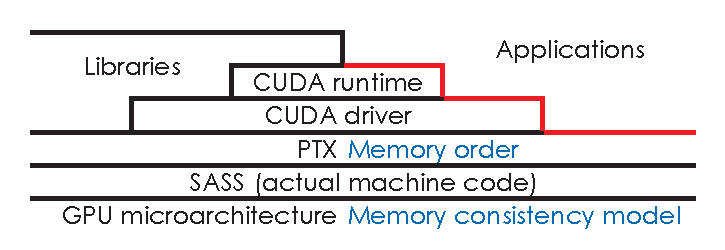
\includegraphics[width=\linewidth]{images/swstack.eps}
            \caption{The GPU software stack.}
            \label{fig:swstack}
        \end{subfigure}
        \vfill
        \begin{subfigure}[b]{\linewidth}
            \centering
            \includegraphics[width=\linewidth]{images/h100.jpg}
            \caption{Hardware schematic of the NVIDIA Hopper H100 GPU.}
            \label{fig:h100}
        \end{subfigure}
    \end{subfigure}
    \hspace{10pt} %\hfill
    \begin{subfigure}[b]{0.47\linewidth}
        \centering
        \includegraphics[width=\linewidth]{images/ptx.eps}
        \caption{Snippets of the PTX virtual ISA.}
        \label{fig:ptx}
    \end{subfigure}
    %\caption{}
    %\label{}
\end{figure}

Fig.~\ref{fig:ptx} presents the format of PTX virtual ISA with memory- and synchronization-related instructions as examples \cite{ptx}. An instruction is led by an \textit{opcode}; following are a few fields called \textit{directives}; an instruction operates on the trailing operands separated by commas (\verb|,|'s). A directive \verb|.xxx| is led by a dot (\verb|.|). Table \ref{table:ptx} elaborates on various directives in company of an opcode.


\begin{table}[H]
    \centering
    \begin{tabular}{llll}
    \toprule
    Field & Name & Description & Possible values \\
    \hline
    \verb|.ss| & State space & \makecell[l]{Level of memory hierarchy that\\an instruction operates on} & \verb|.global| for GPU DRAM, $\cdots$\\
    \verb|.cop| & Cache operator & Cache access pattern & \verb|.cg| for cache at \textit{global} level, $\cdots$\\
    \verb|.scope| & Memory scope & \makecell[l]{Scope where the memory order\\applies} & \makecell[l]{\texttt{.cta} for intra-block consistency,\\$\cdots$}\\
    \verb|.order| & Memory order & & \verb|.relaxed| for \texttt{ld}/\texttt{st}, $\cdots$\\
    \verb|.vec| & Vector type & Level of vectorized memory access & \verb|.v2| for 2-element access, $\cdots$\\
    \verb|.type| & Data type & & \makecell[l]{\texttt{.b16} for half-precision floating\\point number, $\cdots$}\\
    \bottomrule
    \end{tabular}
    \caption{Explanation of PTX directives.}
    \label{table:ptx}
\end{table}

Fig.~\ref{fig:swstack} presents the software stack of NVIDIA GPUs. Touching edges are the interfaces exposed by a lower layer to an adjacent higher layer to utilize its functionalities. All GPU code compiles to PTX and then SASS. The multi-GPU barrier (listing \ref{lst:barrier}) in NVIDIA TensorRT-LLM \cite{trt-llm} includes a runtime API invocation (\verb|__syncthreads();|), driver call (\verb|tidx| and \verb|bidx|), and \verb|inline|d PTX assembly (\verb|asm volatile|). They are the \textcolor{red}{red} edges in Fig.~\ref{fig:swstack}.

\subsection{Axiomatic MCM}
\label{sec:mcm}

%This section first introduces the concept of a Memory Consistency Model (MCM). It then provides an overview of axiomatic MCM, a formalization of MCM. Finally, it presents how PTX's MCM is formalized in \cite{ptx-mcm}.

A MCM is a formal specification that defines the behavior of memory operations in a computer system, particularly in the context of concurrent programs. MCMs are defined at both the hardware and programming language levels. A hardware MCM, such as \textit{total store order} (TSO) on \verb|x86_64| CPUs and \textit{sequential consistency} (SC), specifies how memory operations are ordered and observed by different processors in a multi-core system. A language-level MCM, more frequently called memory order, e.g., RC11 \cite{rc11}, specifies how memory operations should appear to execute in a concurrent program, abstracting away subtleties of the underlying hardware. PTX defines its own MCM as a virtual ISA. It is considered a language-level memory order because it does not directly map to hardware implementation.

An \textit{axiomatic} MCM provides an approach to rigorously modeling MCM. It is usually developed in 3 stages.

\begin{enumerate}
    \item \textbf{Control-flow semantics.} This stage involves mapping each instruction to mathematical objects, allowing the definition of control-flow semantics for a multi-threaded program. This process translates instructions into events, such as memory or register accesses, and establishes \textit{relations} like \textit{program order} ($po$) and dependencies. Fig.~\ref{fig:control-flow} shows the control-flow semantics of a multi-threaded program that implements the \textit{message passing} pattern (Fig.~\ref{fig:original-program}). 
    \item \textbf{Candidate \textit{executions}.} From the control-flow semantics, a set of candidate executions is constructed. Each candidate execution represents a potential dataflow of the program, indicating possible communications between different threads. This involves defining relations over memory events, such as the relation \textit{read from} ($rf$), which specifies the source of a read, and \textit{coherence order} ($co$), which orders writes. Fig.~\ref{fig:dataflow} shows all potential dataflows of Fig.~\ref{fig:original-program}.
    \item \textbf{Constraint specification.} This stage determines the validity of candidate executions. It uses axioms, often based on acyclicity or irreflexivity of relations, to filter invalid executions. For example, a candidate execution will be invalidated if it contains a cycle of specific relations:
    $$
    \verb|acyclic|\Big(\big(morally\_strong \cap (rf \cup co \cup fr)\big) \cup po\_loc\Big)
    $$
    The MCM is thus uniquely defined by a set of axioms, hence the name axiomatic MCM. 
\end{enumerate}

\begin{figure}[H]
    \centering
    \begin{subfigure}[b]{0.3\linewidth}
        \centering
        \begin{subfigure}[b]{\linewidth}
            \centering
            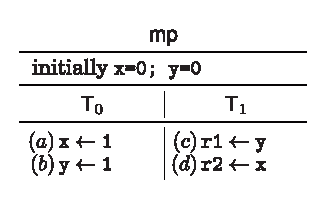
\includegraphics[width=\linewidth]{images/mp.eps}
            \caption{A multithreaded program implementing a message passing pattern.}
            \label{fig:original-program}
        \end{subfigure}
        \vfill
        \begin{subfigure}[b]{\linewidth}
            \centering
            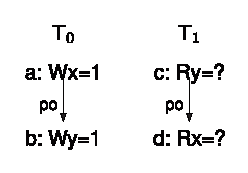
\includegraphics[width=0.8\linewidth]{images/mp_control.eps}
            \caption{Control-flow semantics for the message passing pattern of \ref{fig:original-program}.}
            \label{fig:control-flow}
        \end{subfigure}
    \end{subfigure}
    \hspace{10pt} %\hfill
    \begin{subfigure}[b]{0.5\linewidth}
        \centering
        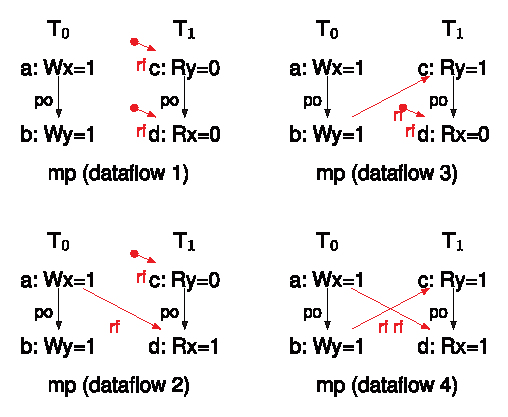
\includegraphics[width=\linewidth]{images/mp_data.eps}
        \caption{All possible dataflow semantics for the control-flow semantics given in \ref{fig:control-flow}.}
        \label{fig:dataflow}
    \end{subfigure}
    \caption{The process of developing an axiomatic MCM using message passing pattern as an example.}
    \label{fig:axiomatic-example}
\end{figure}

Using the same approach, \cite{ptx-mcm} derived the axiomatic MCM of PTX from PTX documentation prose \cite{ptx}. Although CUDA/PTX extends C++, the PTX MCM differs significantly from the that of C++. Specifically, the GPU programming model introduces the concept of scope and employs memory instructions and synchronization primitives with explicit memory order semantics (\verb|.order| in Table \ref{table:ptx}).

We first give an \textbf{intuitive} description of PTX MCM. The \fcolorbox{yellow}{yellow}{highlighted} opcodes and directives in Fig.~\ref{fig:ptx} participates in PTX MCM definition, e.g, \verb|ld|\textcolor{gray}{\texttt{.weak}}, \verb|st.release|, and \verb|fence.sc|.
%Notably, the instructions \verb|ld| and \verb|st| are followed by qualifiers such as \verb|weak|, \verb|relaxed|, \verb|release|, and \verb|acquire|.
These qualifiers impart different semantics to the memory instructions. For example, while the PTX MCM allows\verb|ld|\textcolor{gray}{\texttt{.weak}} to bypass \verb|st|\textcolor{gray}{\texttt{.weak}}, it is prohibited if they are qualified with \verb|.relaxed|. Additionally, all memory instructions preceding \verb|st.release| must be visible to a thread if the result of that \verb|st.release| is visible. The \verb|.scope| directive defines the range within which its semantics are guaranteed.

We now introduce the \textbf{axiomatic} definition of PTX MCM. We do not attempt to provide a comprehensive description as in \cite{ptx-mcm}. Instead, we highlight the notable differences between the axiomatic PTX MCM and other axiomatic MCMs. The goal is to brief readers of the former via comparison.

The PTX MCM applies different rules to memory instructions based on their qualifiers. This necessitates a new set of relations that encodes the qualifiers, allowing the axiomatic MCM to handle them in a unified manner.
%This is achieved with the concept of \textit{morally strong}.
Two operations as \textit{morally strong} relative to each other if each operation is strong (not \verb|.weak|) and specifies a scope that includes the thread executing the other operation.
PTX also incorporates a unique spectrum of scoped synchronization mechanisms because it is not \textit{multi-copy atomic} (simply put, the \textit{store buffering} effect). The three forms of synchronization are the release-acquire pattern, barrier synchronization, and thread fence (corresponding to \verb|__threadfence()| or \verb|__threadfence_system()| in CUDA). These are represented in the axiomatic model using the relation \textit{synchronize with} (\textit{sw}). The \textit{causality} relation extends \textit{sw} and is defined as repetitive composition of \textit{sw} and $po$. Fig.~\ref{fig:ptx-relations} lists all relations in the PTX MCM.

Building on top of the above relations, \cite{ptx-mcm} introduces several axioms that uniquely define the PTX MCM, focusing on how memory operations are ordered and observed. A key component is \textit{causality}, which provides guarantee on the order of memory requests. This axiom states that if a read follows an overlapping write in causality order, then it cannot be from any write accessed by both the read and a subsequent write. This prevents inconsistency and enforces a coherent view of memory across threads, maintaining the integrity of concurrent execution. We will use this axiom towards a formal proof in section \ref{sec:formal}. Fig.~\ref{fig:ptx-axioms} lists all axioms.

\begin{figure}[H]
    \centering
    \begin{subfigure}[b]{0.45\linewidth}
        \centering
        \begin{subfigure}[b]{\linewidth}
            \centering
            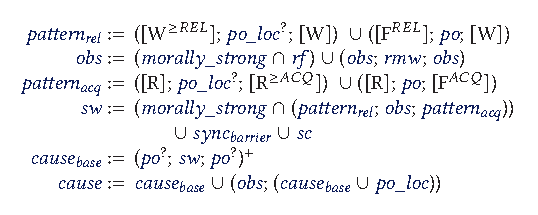
\includegraphics[width=\linewidth]{images/relations.eps}
            \caption{PTX memory model relations.}
            \label{fig:ptx-relations}
        \end{subfigure}
        \vfill
        \begin{subfigure}[b]{\linewidth}
            \centering
            \includegraphics[width=0.55\linewidth]{images/dgx.png}
            \caption{The NVIDIA DGX platform.}
            \label{fig:dgx}
        \end{subfigure}
    \end{subfigure}
    \hspace{10pt} %\hfill
    \begin{subfigure}[b]{0.45\linewidth}
        \centering
        \includegraphics[width=\linewidth]{images/axioms.eps}
        \caption{PTX memory model axioms.}
        \label{fig:ptx-axioms}
    \end{subfigure}
    %\caption{}
    %\label{}
\end{figure}

\subsection{Multi-GPU synchronization}

Multi-GPU synchronization is prevalent in nowadays LLM inference frameworks. To satisfy the \textit{tail latency} requirements --- particularly \textit{time to first token} (TTFT) --- enforced by the \textit{service-level agreement} (SLA), the frameworks employ \textit{tensor parallelism} (TP) and distribute sub-matrices of the weights and \textit{KV cache} among interconnected GPUs. The GPUs keep such data in sync by performing collective communication. Our multi-GPU barrier is part of a larger \textit{all-reduce} kernel; all-reduce is one of the collective communication primitives. While libraries such as NVIDIA NCCL already implemented tree and ring all-reduce operations via \texttt{ncclAllReduce} \cite{nccl}, they require logarithmic and linear complexity, respectively, in communication steps. TensorRT-LLM \texttt{customAllReduce} improves such complexity to $O(1)$ \cite{customallreduce}. A single communication step amounts to synchronizing all interconnected GPUs, and \textit{barrier synchronization} is one of the commonest concurrency constructs in GPU software.

\subsubsection{Shared-memory abstraction}

Fig.~\ref{fig:dgx} illustrates an NVIDIA DGX \textit{node} for LLM inference workloads \cite{dgx}. At the bottom are 4 NVLink network switches (NVSwitches), which provide coherent interconnection between GPUs \cite{nvswitch}. The NVLink interconnection protocol provides \verb|ld|/\verb|st| semantics, so accessing DRAM of another GPU simplifies to ordinary memory access with extra latency penalty compared to local DRAM access. NVSwitches provide \textit{shared-memory} abstraction for all interconnected GPUs via GPUDirect Peer to Peer \cite{gdp2p}. In essence, multi-GPU synchronization becomes a shared-memory synchronization problem.

\section{Intuition}
\label{sec:intuition}

\begin{figure}[H]
    \centering
    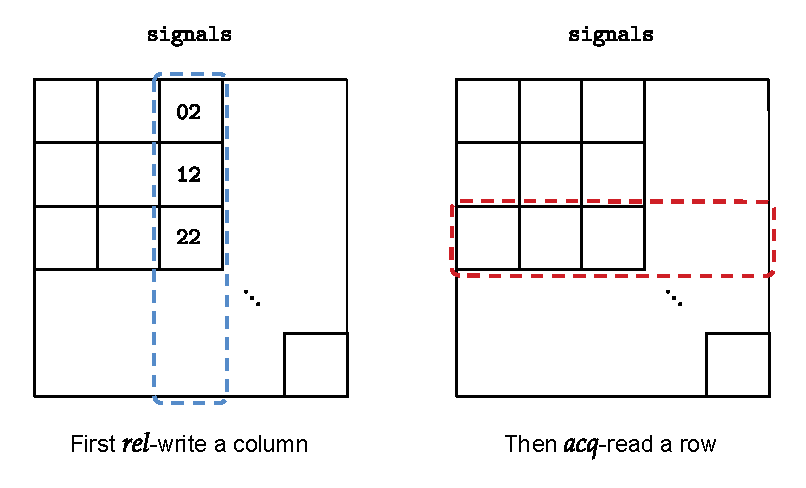
\includegraphics[width=0.7\linewidth]{images/intuition.eps}
    \caption{Intuition behind \texttt{multi\_gpu\_barrier}.}
    \label{fig:intuition}
\end{figure}

% replace figure references !! 
% some slight re-write needed. 
The multi-GPU barrier in Listing~\ref{lst:barrier} relies on two key ideas to ensure that \textit{no GPU} advances until \textit{every GPU} signals it has reached the same point: (1) each GPU’s \textit{block0} broadcasts a flag to every other GPU by writing to shared memory, and (2) every GPU checks that every peer’s flag has been set before proceeding. Although the explanation is described at the GPU level, the underlying implementation occurs at the thread-block level. This section explains why the barrier is effective and briefly illustrates the role of PTX \verb|release|/\verb|acquire|.

Within each GPU, threads in the \textit{leader block} (\texttt{bidx == 0}) writes a \texttt{flag} to a shared array \texttt{signals}. This write uses the PTX directive \texttt{st.global.release}, ensuring that all prior writes in the program order are made visible before the \texttt{flag} is stored. One can visualize this as the coordinating block filling out one column in a “grid” of flags, indicating that the GPU has reached the barrier. The position of the write is determined by the \texttt{tidx}, or thread index. All threads on all GPUs then poll another GPU’s flags in a loop. The load uses \texttt{ld.global.acquire}, meaning each polling thread sees all writes released by the corresponding leader block. Collectively, each GPU checks a row in the “grid” to ensure every other GPU has set its flag. 

Local synchronization is still needed to guarantee that GPUs have observed every peer’s \texttt{flag}, as each thread \texttt{acq} only one flag. The \texttt{\_\_syncthreads()} or \texttt{bar.sync} directive (line 51 in listing \ref{lst:barrier} or lines 48 in listing \ref{lst:barrier-ptx}) accomplishes this: it prevents any thread from continuing until the entire thread pool confirms that their \textit{acq}-ed memory location has been written to. Recall that in the first stage, each GPU writes to a column. Thus, \textbf{intra}-GPU synchronization ensures that \textit{every thread in the block} collectively observes the correct remote flags before continuing, for which \textbf{inter}-GPU synchronization follows.

Figure ref{fig:intuition} schematically illustrate these two phases: on the left, one column highlights the \texttt{release} from threads in the leader block on a GPU writing to shared memory, and on the right, one row emphasizes how every thread block polls a different peer (GPU)'s \texttt{flag} through \texttt{acquire}. One has see how under this model, \textit{acq}-reads from one GPU would depend on \textit{rel}-writes from all other GPUs.

At a more granular level, indexing is completed using the reserved keywords \texttt{tidx}, and \texttt{bidx}, as well as shared memory \texttt{signals}. These are provided as parameters to the barrier code in Listing~\ref{lst:barrier}. \texttt{signals} is an array of pointers to buffers that store flags which represent the barrier. Note that the presence of \texttt{offset} allows for repeated calls to the barrier. Conceptually, it forms a shared 2D grid (\verb|[world_size, world_size]|). \texttt{world\_size} denotes the total number of GPUs participating in the synchronization. Each GPU is assigned a unique \texttt{local\_rank} in the range [0, \texttt{world\_size}-1]. \texttt{local\_rank} is the identifier of the current GPU within the group of \texttt{world\_size} GPUs. In the write phase, \texttt{local\_rank} determines which column in \texttt{signals} is filled. In the read phase, \texttt{local\_rank} helps locate the correct row to poll from other GPUs. Each thread performs a \textit{acq}-read on one location and possibly a \textit{rel}-write on one location.


\section{Effectiveness of \texttt{multi\_gpu\_barrier}}
\label{sec:proof}

\begin{table}[H]
    \centering
    \begin{tabular}{lll}
    \toprule
    \makecell[c]{Item} & \multicolumn{2}{c}{Content}\\
    \hline
    Assumption 1 & Intra-GPU synchrony & \makecell[l]{Blocks in the kernel immediately before \texttt{multi\_gpu\_ba}-\\\texttt{rrier} are properly synchronized, such that all threads\\of all blocks in the kernel immediately after \texttt{multi\_gpu}-\\\texttt{\_barrier} on any GPU have the same view of data local\\to the GPU.}\\
    \arrayrulecolor{gray}\hline\arrayrulecolor{black}
    Theorem 1 & Liveness & \makecell[l]{All threads on all GPUs eventually \textit{leave} \texttt{multi\_gpu\_ba}-\\\texttt{rrier}.}\\
    Theorem 2 & Barrier completion & \makecell[l]{Define block 0 to be the \textit{leader} of all blocks from a ker-\\nel on a GPU. If at least 1 leader \textit{enters} the barrier in the\\${i_{y+2}}^\text{th}$ invocation, then all blocks in the ${i_y}^\text{th}$ invocation\\have \textit{left} the barrier.}\\
    Theorem 3 & Mutual progress & \makecell[l]{Any read ensuing the barrier in $po$ must “see” the data\\written before the barrier in $po$.}\\
    \bottomrule
    \end{tabular}
    \caption{Assumption and theorems to prove the effectiveness of \texttt{multi\_gpu\_barrier}.}
    \label{table:proof-sketch}
\end{table}

We first state the assumption and theorems to prove \textbf{verbally} in Table \ref{table:proof-sketch}. Section \ref{sec:empirical} demonstrates a litmus test generator as an \textbf{empirical} proof. We reiterate the items \textbf{formally} in section \ref{sec:formal} and then outline a \textbf{formal} proof.

\subsection{Empirical proof with litmus tests}
\label{sec:empirical}

As a first step in verification, we perform an empirical analysis of the barrier and synthesized \textbf{litmus} tests to perform verifications under scope. This serves as the basis for further formal proofs in the next section. Litmus tests are concise concurrent code snippets that illustrate or stress specific aspects of a memory consistency model, allowing one to observe potential reorderings or violations under different execution paths. They are a standard tool in verifying whether a design respects a given memory model.

Thus, we manually constructed a simplified version of the barrier (listing \ref{lst:litmus-simple}), where \texttt{offset} and other calculations are precomputed. A verification specification is appended based on the conditions and theorems in table  \ref{table:proof-sketch}. The litmus test is then fed through \textsc{Dat3M}~\cite{unified-analysis} to verify live-ness and the specification. \textsc{Dat3M} is a framework for concurrency testing and model checking in relaxed memory systems; it provides automated checks for correctness properties (e.g., deadlock freedom, reachability) under various memory consistency models. Using this technique, we were able to verify the theorems for a system of two kernels, each with one block and two threads.

We expanded this by writing a Python script that automates the generation of litmus tests with user-configurable settings such as GPU count, grid size, and block size. In this way, we obtained broad coverage of a finite but practically relevant design space. Our source code for this generator, as well as sample litmus tests are available on Github \cite{gpubar}.

These tests confirm that the multi-GPU barrier exhibits the expected memory ordering semantics and does not break under interleavings introduced by the relaxed PTX MCM. We observed no unexpected data races or deadlocks in the tested configurations, corroborating the theoretical assertions of the NVIDIA PTX memory consistency model. However, due to the nature of Dat3M as a state reachability based tool, this type of testing does not scale linearly with the number of threads configured in litmus tests. It is thus necessary to follow with a formal proof.   
% TODO: time vs "scale" plot
% TODO: does not scale

\subsection{Formal proof with MCM and concurrency theorems}
\label{sec:formal}

\noindent For convenience, identify a thread by ${(\text{GPU ID}, b, t)}^k$ for some block index (\verb|bidx|) $b$, thread index (\verb|tidx|) $t$, and kernel function $k$. $k$ defaults to \verb|multi_gpu_barrier|; we omit $k$ unless running other kernels.

\textcolor{white}{delimiter}

\noindent\textbf{Assumption 1.} Intra-GPU synchrony: if $k_1 \xrightarrow[]{po} \verb|multi_gpu_barrier| \xrightarrow[]{po} k_2$ and $W_{{(m,b,t)}^{k_1}} \xrightarrow[]{po} \verb|multi_gpu_barrier| \xrightarrow[]{po} R_{{(\textcolor{blue}{m},b',t')}^{k_2}}$, then $W_{{(m,b,t)}^{k_1}} \xrightarrow[]{rf} R_{{(m,b',t')}^{k_2}}$.

The assumption addresses \textbf{intra}-GPU synchronization whereas \verb|multi_gpu_barrier| targets \textbf{inter}-GPU data synchrony. This assumption is practical. The reasons are two-fold. \textbf{First}, it is the kernel immediately before \verb|multi_gpu_barrier| (\verb|inlined| to TensorRT-LLM, say, \verb|oneShotAllReduceKernel|) that keeps data in sync. A matrix multiplication (GEMM) kernel usually precedes the barrier in TP, and intra-GPU inter-block data synchrony is a cirtical concern for GEMM kernels. \textbf{Second}, we enforce this property on the kernel ensuing the barrier rather than \verb|multi_gpu_barrier| itself. This will leave enough time for memory requests preceding the barrier to complete even with \textit{programmatic dependent launch} \cite{cuda}. The barrier only eyes inter-GPU synchronization.

\begin{center}
$\cdots \xrightarrow[]{po} k_1~\text{(GEMM in TP)} \xrightarrow[]{po} \texttt{multi\_gpu\_barrier} \xrightarrow[]{po} k_2 \xrightarrow[]{po} \cdots$
\end{center}

Unlike a \textit{mutex} lock, which guards a \textit{critical section }, barrier synchronization itself does not guard nor use shared data. GPU-local data must be synchronized by the end of \verb|multi_gpu_barrier|, but there is no such restriction in its beginning.

\noindent\textcolor{gray}{\hrulefill}
\vspace{4pt}

\noindent We first prove the following theorems for 2 interconnected GPUs. Section \ref{sec:induction} applies induction to generalize the theorems to an arbitrary number of GPUs connected by NVLink. \underline{The proof heavily} \underline{uses Fig.~\ref{fig:ptx-relations}. and Fig.~\ref{fig:ptx-axioms}.}

\textcolor{white}{delimiter}

\noindent\textbf{Theorem 1.} \textit{Liveness} is also known as \textit{deadlock freedom}.

\noindent\textbf{Proof.} Define a thread \textit{leaves} the barrier when it finishes executing \verb|bar.sync| (last effective line of listing \ref{lst:barrier-ptx}). A block \textit{leaves} the barrier when all threads leave the barrier. Liveness is satisfied if all blocks on all GPUs leave the barrier. It suffices to prove that no thread is stuck at the \verb|while| loop (line 46 in listing \ref{lst:barrier} or lines 42 -- 45 in listing \ref{lst:barrier-ptx}). The \verb|st| request (line 32 of listing \ref{lst:barrier-ptx}) eventually \textit{commits}, so \verb|ld.acquire| eventually sees the correct flag value. Hence, a thread eventually exits the loop. Liveness is trivially satisfied.

\begin{flushright}
$\square$
\end{flushright}

\noindent\textbf{Theorem 2.} Barrier completion. For convenience, denote \verb|multi_gpu_barrier| as $\mathbf{B}$. Define a sequence $i_0, i_1, \cdots, i_y, i_{y+1}, i_{y+2}, \cdots, i_x$ such that any adjacent $i_\_$'s have different oddity. $i_\_$ serves as the flag value of the invocation sequence of $\mathbf{B}$. When $i_\_$'s is the natural number sequence ($i_0 = 0, i_1 = 1, \cdots$), the simplest that satisfies the oddity constraint, $\mathbf{B}_{i_0}, \mathbf{B}_{i_1}, \cdots, \mathbf{B}_{i_x}$ simplifies to $\mathbf{B}_0, \mathbf{B}_1, \cdots, \mathbf{B}_y,$ $\mathbf{B}_{y+1}, \mathbf{B}_{y+2}, \cdots, \mathbf{B}_x$, which is a sequence of \verb|multi_gpu_barrier| invocations ($x$ times in total). Define a thread \textit{enters} the barrier when it issues the \verb|st| request (line 32 of listing \ref{lst:barrier-ptx}). A block \textit{enters} the barrier when all threads enter the barrier. Define block 0 to be the \textit{leader} of all blocks in a kernel on a GPU.
If $\mathbf{B}_y \xrightarrow[]{po} \mathbf{B}_{y+1} \xrightarrow[]{po} \mathbf{B}_{y+2}$ and $\exists n,t'$ such that $\texttt{st}_{{(n,0,t')}^{\mathbf{B}_{y\textcolor{blue}{+2}}}}$ is issued, then $\forall m,b,t$, we have $\texttt{bar.sync}_{{(m,b,t)}^{\mathbf{B}_{y}}}$ completed.

\noindent\textbf{Proof.} When $\texttt{st}_{{(n,0,t')}^{\mathbf{B}_{y\textcolor{blue}{+2}}}}$ is dispatched for some $n,t'$, at least 1 leader has entered $\mathbf{B}^{y+2}$. This means all leaders on all GPUs have issued $\texttt{st}_{{(\_,0,\_)}^{\mathbf{B}_{y\textcolor{blue}{+1}}}}$, i.e., have entered $\mathbf{B}_{y+1}$. Otherwise, block $(n,0,\_)$ would not have left the barrier. Now that $\mathbf{B}_y \xrightarrow[]{po} \mathbf{B}_{y+1}$, all threads have left $\mathbf{B}_y$. That is, $\texttt{bar.sync}_{{(m,b,t)}^{\mathbf{B}_{y}}}$ has completed for all $m,b,t$.

\begin{flushright}
$\square$
\end{flushright}

Theorem 2 targets the branch caused by the oddity of the flag value (line 36 of listing \ref{lst:barrier}). \verb|multi_|-\verb|gpu_barrier| adopts \textit{double buffering}, expanding the intuition in section \ref{sec:intuition}, and writes to signal locations in a ping-pong fashion based on the oddity of the flag. We have to make sure the signals are not overwritten when a barrier is not yet completed.

\noindent\textbf{Theorem 3.} Mutual progress: if $k_1 \xrightarrow[]{po} \verb|multi_gpu_barrier| \xrightarrow[]{po} k_2$ and $W_{{(m,b,t)}^{k_1}} \xrightarrow[]{po} \verb|multi_gpu_|$-$\verb|barrier| \xrightarrow[]{po} R_{{(m,b',t')}^{k_2}}$, then $W_{{(m,b,t)}^{k_1}} \xrightarrow[]{rf} R_{{(\textcolor{red}{n},b',t')}^{k_2}}$.

\noindent\textbf{Proof.} There are 3 branchs in \verb|multi_gpu_barrier|. We already addressed the ternary operator (line 36 of listing \ref{lst:barrier}) in \textbf{theorem 2}. There remains 2 \verb|if|'s (lines 30 and 38 of listing \ref{lst:barrier}) to consider, which span 4 scenarios in all executions. They are

\begin{table}[H]
\centering
\begin{tabular}{l|l}
 & Possible values \\\hline
$b$ & $\{0\}, \{1, 2, \cdots, \texttt{gridDim.x}\}$\\
$t$ & $\{0,1\}, \{t_2 | t_2 \geq \texttt{world\_size}\}$
\end{tabular}
\caption{Scenarios to consider to prove theorem 3.}
\label{table:scenarios}
\end{table}

For some memory location, either $W \xrightarrow[]{rf} R$ --- read the previously written value --- or $W \xleftarrow[]{fr} R$ --- read some stale value then write. As mentioned in section \ref{sec:mcm}, for a read to ``see" the previous write, it \textbf{suffices to show that $W \xrightarrow[]{cause} R$} given $W \xrightarrow[]{po} R$. Otherwise, $W \xleftarrow[]{fr} R$ and $W \xrightarrow[]{cause} R$ imply a cycle, violating axiom 6 (Fig.~\ref{fig:ptx-axioms}). We directly prove all scenarios as follows.

\textcolor{white}{delimiter}

\noindent\textbf{Case 1.}

\begin{figure}[H]
    \centering
    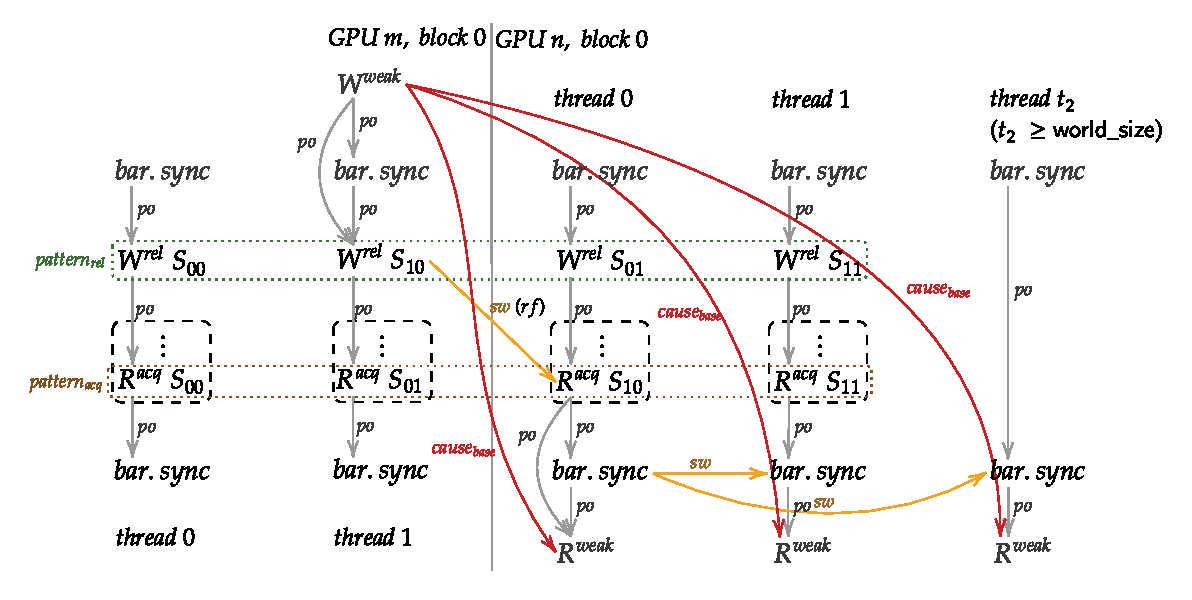
\includegraphics[width=\linewidth]{images/0-0-1—1-0-t.eps}
    \caption{Thread $(m, 0, 1)$ synchronizes with thread $(n, 0, t)$.}
    \label{fig:0-0-1—1-0-t}
\end{figure}

Fig.~\ref{fig:0-0-1—1-0-t} sketches the execution where thread $(m, 0, 0)$ synchronizes with thread $(n, 0, t)$. By \textbf{assumption 1}, threads already have the same view of data local to a GPU, so it does not hurt to add \verb|bar.sync| before $W^{rel}$ (line 32 of listing \ref{lst:barrier-ptx}), before which we manually add a $W^{weak}$ to simulate the result written in the previous GEMM kernel. Likewise, we add a $R^{weak}$ to mimic the cross-GPU read of the all-reduce operaion. We further unroll the \verb|while| loop such that $po$ speaks strictly in terms of instructions executed:

\begin{table}[H]
\centering
\begin{tabular}{c|l}
    Iteration & \makecell[c]{Instruction}\\
    \hline
    0 & \footnotesize{\verb|ld.global.acquire.sys.b32 %r5, [%rd3]|}\\
     & \cellcolor[HTML]{EFEFEF}\footnotesize{\verb|setp.ne.s32 %p4, %r5, % r1|}\\
     & \cellcolor[HTML]{EFEFEF}\footnotesize{\verb|@%p4 bra $L__BB0_4|}\\
    1 & \footnotesize{\verb|ld.global.acquire.sys.b32 %r5, [%rd3]|}\\
     & \cellcolor[HTML]{EFEFEF}\footnotesize{\verb|setp.ne.s32 %p4, %r5, % r1|}\\
     & \cellcolor[HTML]{EFEFEF}\footnotesize{\verb|@%p4 bra $L__BB0_4|}\\
    \vdots & \makecell[c]{\vdots}\\
    $N-1$ & \footnotesize{\verb|ld.global.acquire.sys.b32 %r5, [%rd3]|}\\
     & \cellcolor[HTML]{EFEFEF}\footnotesize{\verb|setp.ne.s32 %p4, %r5, % r1|}\\
     & \cellcolor[HTML]{EFEFEF}\footnotesize{\verb|@%p4 bra $L__BB0_4|}\\
    $N$ & \footnotesize{\verb|ld.global.acquire.sys.b32 %r5, [%rd3]|}
\end{tabular}
\caption{Unrolled instruction execution trace of the \texttt{while} loop. $N$ is finite by \textbf{theorem 1}. Predicate registers (\fcolorbox{mygray}{mygray}{gray background}) do not participate in MCM definition.}
\label{table:loop}
\end{table}

We may safely reduce the instruction trace to a finite sequence of \texttt{ld}'s regulated by $po$. This is because \textit{predicate} registers do not participate in MCM definition. Focus on the last \verb|ld| before the thread exits the loop. This \verb|ld| must read the correct flag value, so $W^{rel} \xrightarrow[]{rf} R^{acq}$ for signal location \verb|10| (We omit the proof of $W^{rel} \xrightarrow[]{rf} R^{acq}$, which is the example in Fig.~5 of \cite{ptx-mcm}). Such a $rf$ relation is also $obs$ because signal \verb|10| are accessed with morally strong instructions (Fig.~\ref{fig:ptx-relations}). Together with ${pattern}_{rel}$ and ${pattern}_{acq}$, we escalate relation $obs$ to $sw$. Therefore, ${cause}_{base}$ regulates the write in thread $(m,0,1)$ and the read in thread $(n,0,0)$. ${cause}_{base}$ itself is $cause$.

Thread $(n,0,0)$ servers as a synchronization ``broker" for threads $(n,0,1)$ and $(n,0,t_2)$ ($t_2 \geq \verb|world_size|$) via the trailing \verb|bar.sync|. All \verb|bar.sync|'s within a block bear a $sw$ relation. ${cause}_{base}$ still applies between the write in thread $(m,0,1)$ and the reads in threads $(n,0,1)$ and $(n,0,t_2)$.

\textcolor{white}{delimiter}

\noindent\textbf{Case 2} differs from case 1 only by \verb|tidx| in GPU $m$ (Fig.~\ref{fig:0-0-0—1-0-t} left).

\begin{figure}[H]
    \centering
    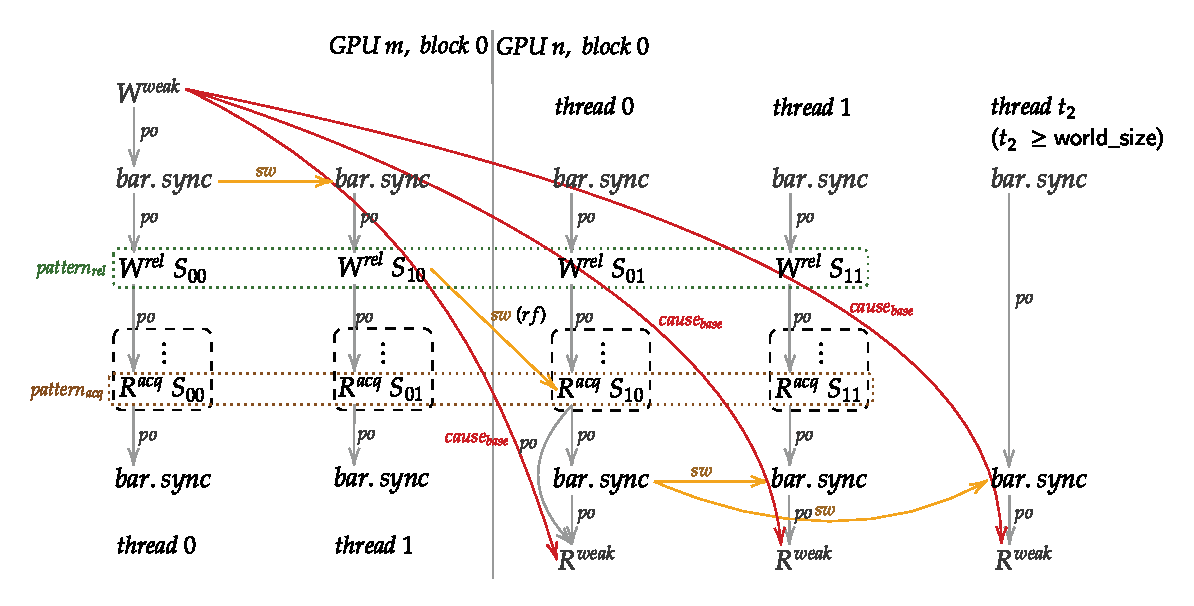
\includegraphics[width=\linewidth]{images/0-0-0—1-0-t.eps}
    \caption{Thread $(m, 0, 0)$ synchronizes with thread $(n, 0, t)$.}
    \label{fig:0-0-0—1-0-t}
\end{figure}

Thread $(m,0,1)$ servers as the synchronization broker between thread $(m,0,0)$ and threads $(n,0,t)$. We introduce the broker because they do not share the same signal location. The manually added \verb|bar.sync| before $W^{rel}$ implies a $sw$ relation. ${cause}_{base}$ can be repetitive, so the causality relation persists between thread $(m,0,1)$ and threads $(n,0,t)$.

\textcolor{white}{delimiter}

\noindent\textbf{Case 3} differs from case 2 on the right side of Fig.~\ref{fig:0-0-0—1-1-t}. WLOG, we pick $1$ for any non-zero $b$. A non-leader reads but never writes the signals.

\begin{figure}[H]
    \centering
    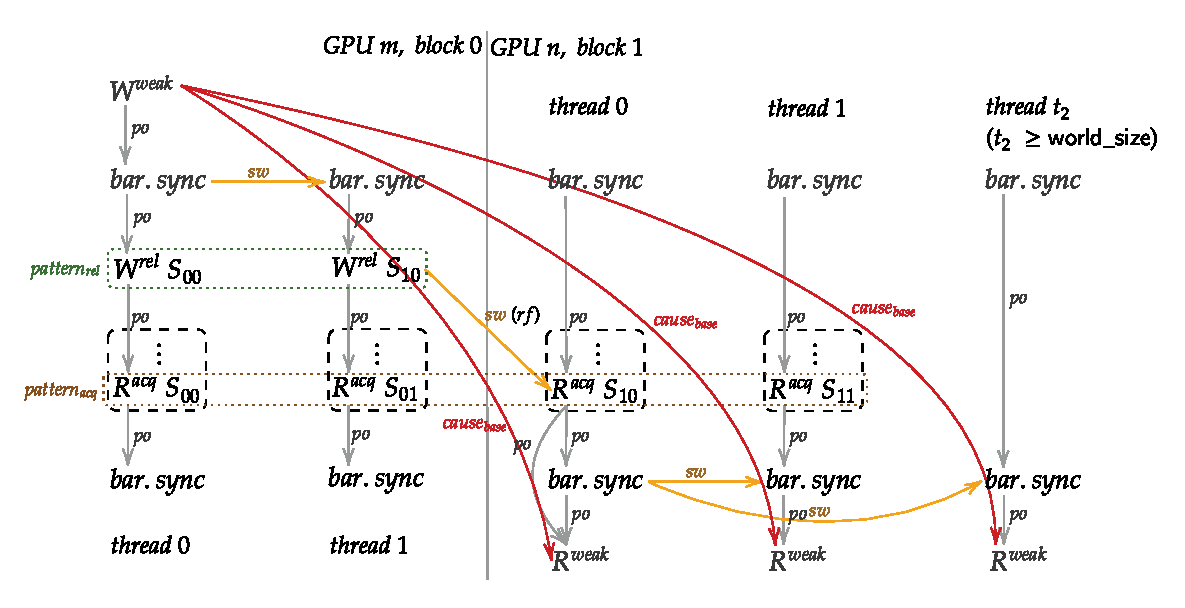
\includegraphics[width=\linewidth]{images/0-0-0—1-1-t.eps}
    \caption{Thread $(m, 0, 0)$ synchronizes with thread $(n, 1, t)$.}
    \label{fig:0-0-0—1-1-t}
\end{figure}

${pattern}_{rel}$ and ${pattern}_{acq}$ remain in this scenario. The absence of \verb|st|'s in non-leaders does not impact the ${cause}_{base}$ relation.

\textcolor{white}{delimiter}

\noindent\textbf{Case 4.}

\begin{figure}[H]
    \centering
    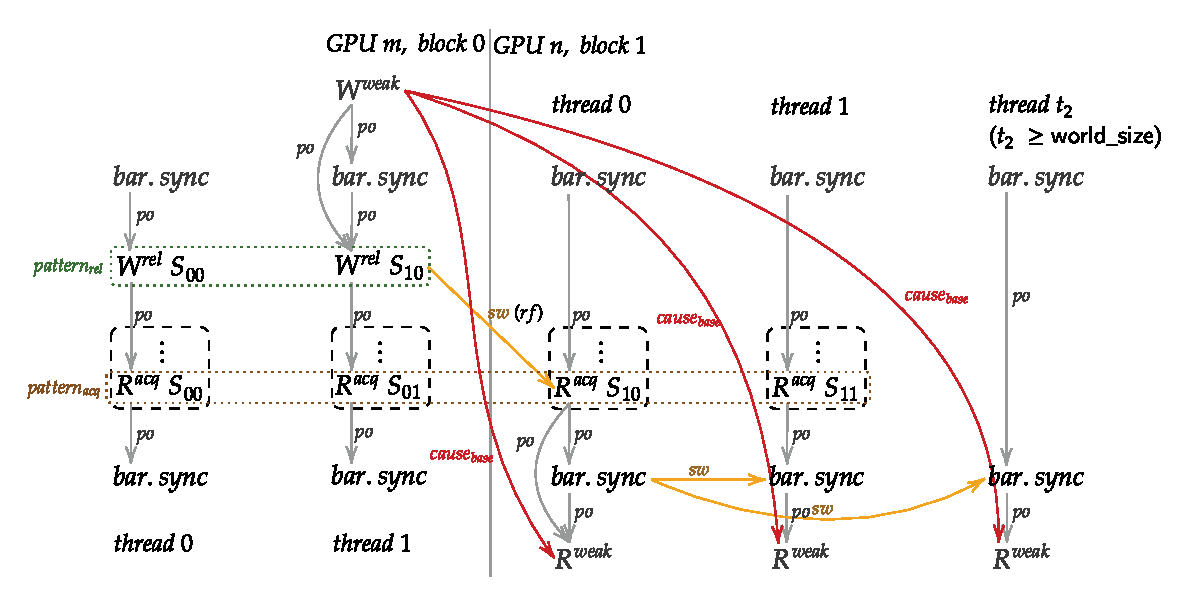
\includegraphics[width=\linewidth]{images/0-0-1—1-1-t.eps}
    \caption{Thread $(m, 0, 1)$ synchronizes with thread $(n, 1, t)$.}
    \label{fig:0-0-1—1-1-t}
\end{figure}

The difference between cases 4 and 3 is analogous to that between cases 1 and 2. We stick to our arguments, and the ${cause}_{base}$ relation is straightforward.

We have shown that $W \xrightarrow[]{cause} R$ (given $W \xrightarrow[]{po} R$) holds in all possible scenarios.

\begin{flushright}
$\square$
\end{flushright}

Theorem 3 states that local computation results, e.g., from a GEMM kernel, are safe for peer GPUs to access. This aligns with TensorRT-LLM \verb|customAllReduce| use cases, where cross-GPU reduction is performed after the barrier.

\subsubsection{Proof by induction}
\label{sec:induction}

We now show that the above theorems hold for any number of intersonnected GPUs.

\begin{figure}[H]
    \centering
    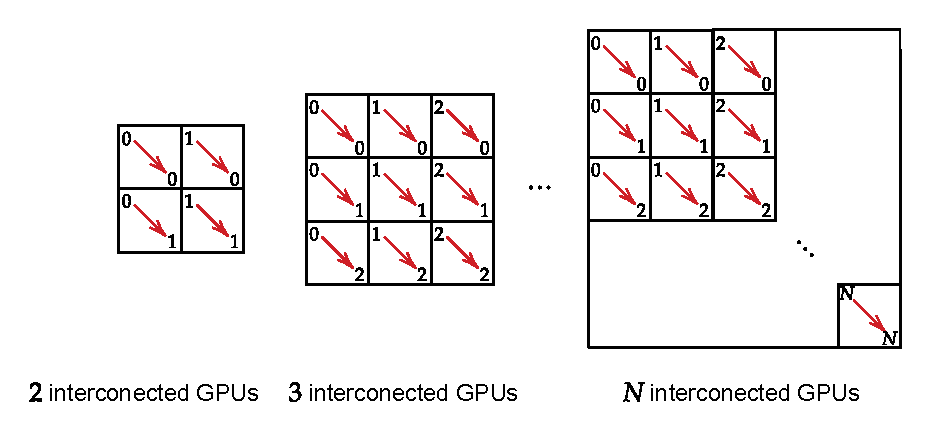
\includegraphics[width=0.75\linewidth]{images/induction.eps}
    \caption{Signals are a square shared-memory memory chunk for \texttt{multi\_gpu\_barrier}.}
    \label{fig:induction}
\end{figure}

\noindent\textbf{Theorem 1'} trivially scales to an arbitrary number of GPUs because all signal location will be eventually written by leaders.\hfill $\square$

\textcolor{white}{delimiter}

\noindent\textbf{Theorem 2'} trivially extends to more interconnected GPUs in light of theorem 1'.\hfill $\square$

\textcolor{white}{delimiter}

\noindent\textbf{Theorem 3'.}

\noindent\textbf{Proof.} Note the concept of synchronization ``broker" in theorem 3. It is essentially a shared signal location a thread writes to and reads from. Thread $(m,0,\_)$ writes to and thread $(n,\_,\_)$ reads from signal location \verb|mn|. The sufficient condition of $W_{{(m,b,t)}^{k_1}} \xrightarrow[]{rf} R_{{(\textcolor{red}{n},b',t')}^{k_2}}$ (given $k_1 \xrightarrow[]{po} \verb|multi_gpu_ba|$-$\verb|rrier| \xrightarrow[]{po} k_2$ and $W_{{(m,b,t)}^{k_1}} \xrightarrow[]{po} \verb|multi_gpu_barrier| \xrightarrow[]{po} R_{{(m,b',t')}^{k_2}}$) is that thread $(m,b,t)$ writes to and thread $(n,b',t')$ reads from some shared memory location, in this case \verb|S[m][n]|. Fig.~\ref{fig:induction} visualizes part of the memory chunk used for barrier synchronization. $m \rightarrow n$ means $W_{{(m,b,t)}^{k_1}} \xrightarrow[]{rf} R_{{(\textcolor{red}{n},b',t')}^{k_2}}$ by accessing this \textit{word}. The memory chunk grows as per the number of interconnected GPUs. Hence, theorem 3 scales to any number of interconnected GPUs.

\begin{flushright}
$\square$
\end{flushright}

In practice, NVIDIA supports up to 288 interconnected GPUs \cite{nvl32,nvl36-72,computex}. There is only a single level of NVSwitch \cite{nvswitch}, so synchronizing dozens of NVLink-connected GPUs will not come with significant latency overhead.

\section{Conclusion}
\label{sec:conclusion}

Multi-GPU synchronization is critical to reduce the latency of collective communication in large
LLM inference. Inference frameworks adopt atomics with memory order semantics for performance, posing challenges for testing and maintanence. Our project unveiled the mechanism of the multi-GPU barrier synchronization (listing \ref{lst:barrier}) in NVIDIA TensorRT-LLM \cite{trt-llm}, both empirically with litmus tests and formally with MCM and concurrency theorems.

%%
%% The next two lines define the bibliography style to be used, and
%% the bibliography file.
\bibliographystyle{ACM-Reference-Format}
\bibliography{references.bib}

\appendix

\section{Multi-GPU barrier}

\subsection{CUDA kernel of the barrier}

\lstset{language=CUDA}
\begin{lstlisting}[caption={\href{https://github.com/NVIDIA/TensorRT-LLM/blob/75057cd036af25e288c004d8ac9e52fd2d6224aa/cpp/tensorrt_llm/kernels/customAllReduceKernels.cu}{\texttt{customAllReduceKernels.cu}} of NVIDIA \href{https://github.com/NVIDIA/TensorRT-LLM/}{\faGithub~TensorRT-LLM}.}, label={lst:barrier}]
static inline __device__ void st_flag_release(uint32_t const& flag, uint32_t* flag_addr)
{
#if __CUDA_ARCH__ >= 700
    asm volatile("st.global.release.sys.b32 [%1], %0;" ::"r"(flag), "l"(flag_addr));
#else
    __threadfence_system();
    asm volatile("st.global.volatile.b32 [%1], %0;" ::"r"(flag), "l"(flag_addr));
#endif
}

///////////////////////////////////////////////////////////////////////////////////

static inline __device__ uint32_t ld_flag_acquire(uint32_t* flag_addr)
{
    uint32_t flag;
#if __CUDA_ARCH__ >= 700
    asm volatile("ld.global.acquire.sys.b32 %0, [%1];" : "=r"(flag) : "l"(flag_addr));
#else
    asm volatile("ld.global.volatile.b32 %0, [%1];" : "=r"(flag) : "l"(flag_addr));
#endif
    return flag;
}

///////////////////////////////////////////////////////////////////////////////////

__inline__ __device__ void multi_gpu_barrier(uint32_t** signals, uint32_t const flag,
    size_t const local_rank, size_t const world_size, int const tidx, int const bidx)
{
    // After this function, at least one block in each GPU has reached the barrier
    if (tidx < world_size)
    {
        // we can think of signals having the shape [world_size, world_size]
        // Dimension 0 is the "listening" dimension, dimension 1 is "emitting" dimension

        // Block 0 broadcasts its flag (local_rank on emitting dimension) to all receivers
        size_t offset = (flag % 2) ? world_size : 0;

        if (bidx == 0)
        {
            st_flag_release(flag, signals[tidx] + offset + local_rank);
        }

        // All blocks check that corresponding block 0 on other GPUs have set the flag
        // No deadlock because block #0 is always the first block started
        uint32_t* peer_barrier_d = signals[local_rank] + offset + tidx;
        while (ld_flag_acquire(peer_barrier_d) != flag)
        {
        }
    }

    __syncthreads();
}
\end{lstlisting}

\subsection{PTX snippet of the compiled CUDA kernel}

%\begin{comment}

\lstset{language=PTX}
\begin{lstlisting}[caption={Compiled PTX snippet of listing \ref{lst:barrier}. We used \href{https://docs.nvidia.com/cuda/cuda-compiler-driver-nvcc/}{\texttt{nvcc} \faExternalLinkSquare} v12.6 with the flag \texttt{-O3 -gencode=arch=compute\_90,code=sm\_90}.}, label={lst:barrier-ptx}]
.visible .func multi_gpu_barrier(unsigned int**, unsigned int, unsigned long, unsigned long, int, int)(
        .param .b64 multi_gpu_barrier(unsigned int**, unsigned int, unsigned long, unsigned long, int, int)_param_0,
        .param .b32 multi_gpu_barrier(unsigned int**, unsigned int, unsigned long, unsigned long, int, int)_param_1,
        .param .b64 multi_gpu_barrier(unsigned int**, unsigned int, unsigned long, unsigned long, int, int)_param_2,
        .param .b64 multi_gpu_barrier(unsigned int**, unsigned int, unsigned long, unsigned long, int, int)_param_3,
        .param .b32 multi_gpu_barrier(unsigned int**, unsigned int, unsigned long, unsigned long, int, int)_param_4,
        .param .b32 multi_gpu_barrier(unsigned int**, unsigned int, unsigned long, unsigned long, int, int)_param_5
)
{

        ld.param.u64    %rd4, [multi_gpu_barrier(unsigned int**, unsigned int, unsigned long, unsigned long, int, int)_param_0];
        ld.param.u32    %r1, [multi_gpu_barrier(unsigned int**, unsigned int, unsigned long, unsigned long, int, int)_param_1];
        ld.param.u64    %rd5, [multi_gpu_barrier(unsigned int**, unsigned int, unsigned long, unsigned long, int, int)_param_2];
        ld.param.u64    %rd6, [multi_gpu_barrier(unsigned int**, unsigned int, unsigned long, unsigned long, int, int)_param_3];
        ld.param.s32    %rd1, [multi_gpu_barrier(unsigned int**, unsigned int, unsigned long, unsigned long, int, int)_param_4];
        ld.param.u32    %r2, [multi_gpu_barrier(unsigned int**, unsigned int, unsigned long, unsigned long, int, int)_param_5];
        setp.ge.u64     %p1, %rd1, %rd6;
        @%p1 bra        $L__BB0_5;

        and.b32         %r3, %r1, 1;
        setp.eq.b32     %p2, %r3, 1;
        selp.b64        %rd2, %rd6, 0, %p2;
        setp.ne.s32     %p3, %r2, 0;
        @%p3 bra        $L__BB0_3;

        shl.b64         %rd8, %rd1, 3;
        add.s64         %rd9, %rd4, %rd8;
        add.s64         %rd10, %rd2, %rd5;
        ld.u64  %rd11, [%rd9];
        shl.b64         %rd12, %rd10, 2;
        add.s64         %rd7, %rd11, %rd12;
        st.global.release.sys.b32 [%rd7], %r1;

$L__BB0_3:
        shl.b64         %rd13, %rd5, 3;
        add.s64         %rd14, %rd4, %rd13;
        add.s64         %rd15, %rd2, %rd1;
        ld.u64  %rd16, [%rd14];
        shl.b64         %rd17, %rd15, 2;
        add.s64         %rd3, %rd16, %rd17;

$L__BB0_4:
        ld.global.acquire.sys.b32 %r5, [%rd3];
        setp.ne.s32     %p4, %r5, %r1;
        @%p4 bra        $L__BB0_4;

$L__BB0_5:
        bar.sync        0;
        ret;

}
        {

        }
\end{lstlisting}

%\end{comment}


\subsection{Sample litmus test with verification specification}

%\begin{comment}

\lstset{language=ptx}
\begin{lstlisting}[caption={A sample litmus test with simplified instructions matching listing \ref{lst:barrier-ptx}. Note that predicate registers are not supported, so control flow is facilitated using \texttt{bne}.}, label={lst:litmus-simple}]
PTX MultiGPU Barrier Test
{
  P0:r0=1;
  P1:r0=1;
  P2:r0=1;
  P3:r0=1;
  
  R0C0=1;
  R0C1=1;
  R1C0=1;
  R1C1=1;
  flag=0;
  x=0;
}



  P0@cta 0,gpu 0                    | P1@cta 0,gpu 0                    | 
  st.weak x, 1                      |                                   | 
  st.release.sys R0C0, 0            | st.release.sys R1C0, 0            | 
  LC00:                             | LC10:                             | 
  ld.acquire.sys r0, R0C0           | ld.acquire.sys r0, R0C1           | 
  bne r0, 0, LC00                   | bne r0, 0, LC10                   | 
  bar.cta.sync 0                    | bar.cta.sync 0                    | 
                                    | ld.weak r1, x                     | 

  P2@cta 0,gpu 1                    | P3@cta 0,gpu 1                     ;
                                    |               	       	         ;
  st.release.sys R0C1, 0            | st.release.sys R1C1, 0             ;
  LC20:                             | LC30:                              ;   
  ld.acquire.sys r0, R1C0           | ld.acquire.sys r0, R1C1            ;
  bne r0, 0, LC20                   | bne r0, 0, LC30                    ;
  bar.cta.sync 0                    | bar.cta.sync 0                     ;
                                    |										                 ;
forall
(P1:r1 = 1)

\end{lstlisting}


%%
\end{document}
\endinput
%%
%% End of file `main.tex'.
